% Created by tikzDevice version 0.11 on 2018-10-22 23:26:00
% !TEX encoding = UTF-8 Unicode
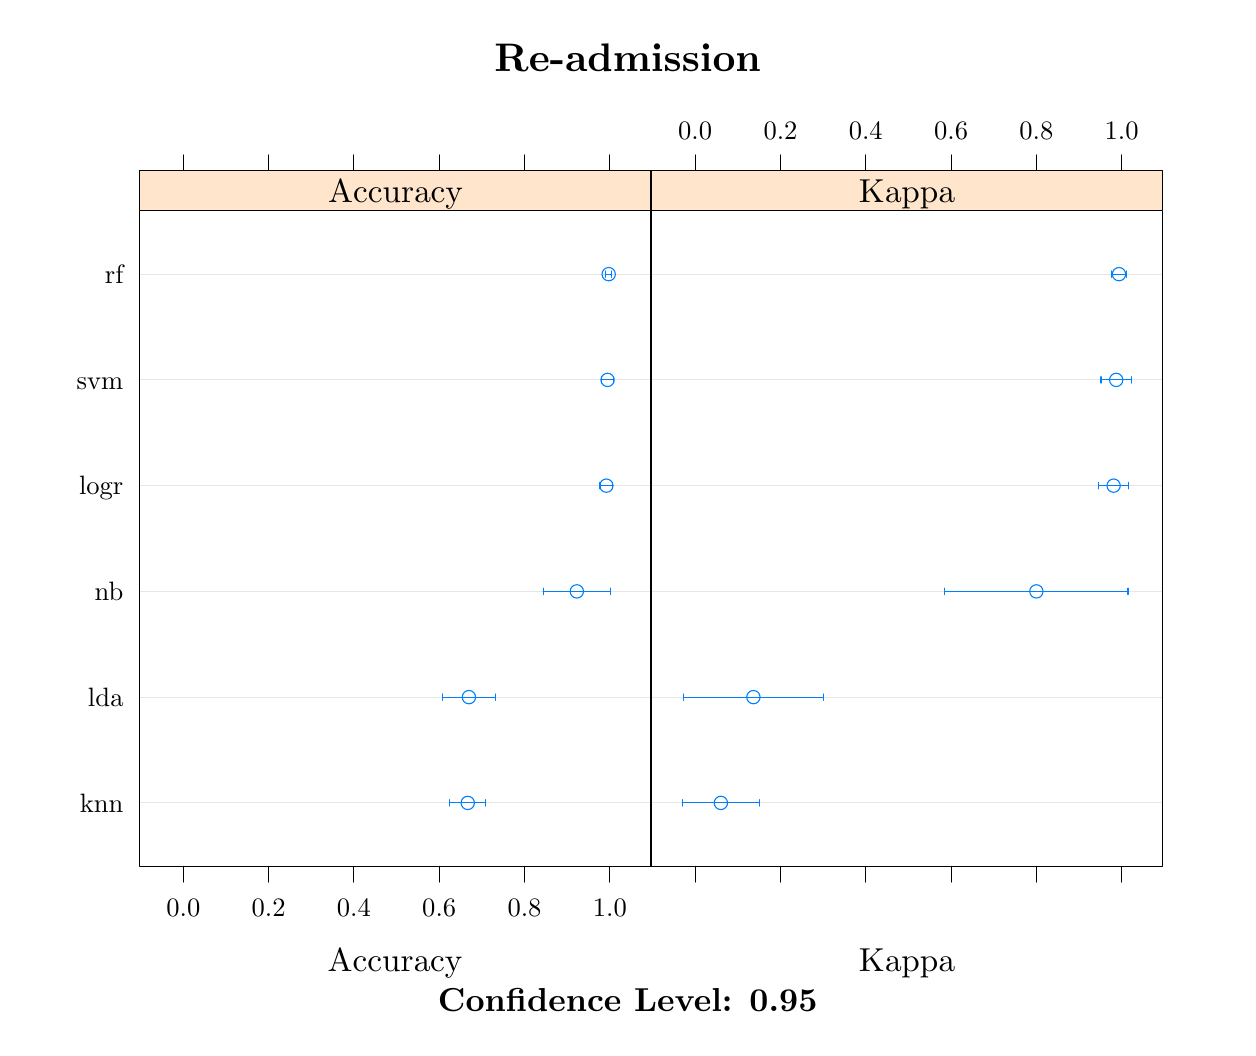
\begin{tikzpicture}[x=1pt,y=1pt]
\definecolor{fillColor}{RGB}{255,255,255}
\path[use as bounding box,fill=fillColor,fill opacity=0.00] (0,0) rectangle (433.62,361.35);
\begin{scope}
\path[clip] (  0.00,  0.00) rectangle (433.62,361.35);

\path[] (  0.00,  0.00) rectangle (433.62,361.35);
\definecolor{drawColor}{RGB}{0,0,0}

\node[text=drawColor,anchor=base,inner sep=0pt, outer sep=0pt, scale=  1.44] at (216.81,345.39) {\bfseries Re-admission};
\end{scope}
\begin{scope}
\path[clip] (  0.00,  0.00) rectangle (433.62,361.35);
\definecolor{drawColor}{RGB}{0,0,0}

\node[text=drawColor,anchor=base,inner sep=0pt, outer sep=0pt, scale=  1.20] at (216.81,  6.02) {\bfseries Confidence Level: 0.95};
\end{scope}
\begin{scope}
\path[clip] (  0.00,  0.00) rectangle (433.62,361.35);
\definecolor{drawColor}{RGB}{0,0,0}

\node[text=drawColor,anchor=base,inner sep=0pt, outer sep=0pt, scale=  1.20] at (132.76, 20.33) {Accuracy};

\node[text=drawColor,anchor=base,inner sep=0pt, outer sep=0pt, scale=  1.20] at (317.71, 20.33) {Kappa};
\end{scope}
\begin{scope}
\path[clip] (  0.00,  0.00) rectangle (433.62,361.35);
\definecolor{drawColor}{RGB}{0,0,0}

\path[draw=drawColor,line width= 0.4pt,line join=round,line cap=round] ( 56.24,309.66) -- ( 56.24,315.35);

\path[draw=drawColor,line width= 0.4pt,line join=round,line cap=round] ( 87.07,309.66) -- ( 87.07,315.35);

\path[draw=drawColor,line width= 0.4pt,line join=round,line cap=round] (117.89,309.66) -- (117.89,315.35);

\path[draw=drawColor,line width= 0.4pt,line join=round,line cap=round] (148.71,309.66) -- (148.71,315.35);

\path[draw=drawColor,line width= 0.4pt,line join=round,line cap=round] (179.54,309.66) -- (179.54,315.35);

\path[draw=drawColor,line width= 0.4pt,line join=round,line cap=round] (210.36,309.66) -- (210.36,315.35);
\end{scope}
\begin{scope}
\path[clip] (  0.00,  0.00) rectangle (433.62,361.35);
\definecolor{drawColor}{RGB}{0,0,0}

\node[text=drawColor,anchor=base east,inner sep=0pt, outer sep=0pt, scale=  0.96] at ( 34.58, 77.92) {knn};

\node[text=drawColor,anchor=base east,inner sep=0pt, outer sep=0pt, scale=  0.96] at ( 34.58,116.13) {lda};

\node[text=drawColor,anchor=base east,inner sep=0pt, outer sep=0pt, scale=  0.96] at ( 34.58,154.34) {nb};

\node[text=drawColor,anchor=base east,inner sep=0pt, outer sep=0pt, scale=  0.96] at ( 34.58,192.55) {logr};

\node[text=drawColor,anchor=base east,inner sep=0pt, outer sep=0pt, scale=  0.96] at ( 34.58,230.76) {svm};

\node[text=drawColor,anchor=base east,inner sep=0pt, outer sep=0pt, scale=  0.96] at ( 34.58,268.97) {rf};
\end{scope}
\begin{scope}
\path[clip] (  0.00,  0.00) rectangle (433.62,361.35);
\definecolor{drawColor}{RGB}{0,0,0}

\path[draw=drawColor,line width= 0.4pt,line join=round,line cap=round] ( 56.24, 58.30) -- ( 56.24, 52.61);

\path[draw=drawColor,line width= 0.4pt,line join=round,line cap=round] ( 87.07, 58.30) -- ( 87.07, 52.61);

\path[draw=drawColor,line width= 0.4pt,line join=round,line cap=round] (117.89, 58.30) -- (117.89, 52.61);

\path[draw=drawColor,line width= 0.4pt,line join=round,line cap=round] (148.71, 58.30) -- (148.71, 52.61);

\path[draw=drawColor,line width= 0.4pt,line join=round,line cap=round] (179.54, 58.30) -- (179.54, 52.61);

\path[draw=drawColor,line width= 0.4pt,line join=round,line cap=round] (210.36, 58.30) -- (210.36, 52.61);

\node[text=drawColor,anchor=base,inner sep=0pt, outer sep=0pt, scale=  0.96] at ( 56.24, 40.30) {0.0};

\node[text=drawColor,anchor=base,inner sep=0pt, outer sep=0pt, scale=  0.96] at ( 87.07, 40.30) {0.2};

\node[text=drawColor,anchor=base,inner sep=0pt, outer sep=0pt, scale=  0.96] at (117.89, 40.30) {0.4};

\node[text=drawColor,anchor=base,inner sep=0pt, outer sep=0pt, scale=  0.96] at (148.71, 40.30) {0.6};

\node[text=drawColor,anchor=base,inner sep=0pt, outer sep=0pt, scale=  0.96] at (179.54, 40.30) {0.8};

\node[text=drawColor,anchor=base,inner sep=0pt, outer sep=0pt, scale=  0.96] at (210.36, 40.30) {1.0};
\end{scope}
\begin{scope}
\path[clip] ( 40.28, 58.30) rectangle (225.23,295.21);
\definecolor{drawColor}{RGB}{230,230,230}

\path[draw=drawColor,line width= 0.4pt,line join=round,line cap=round] ( 40.28, 81.22) -- (225.23, 81.22);

\path[draw=drawColor,line width= 0.4pt,line join=round,line cap=round] ( 40.28,119.44) -- (225.23,119.44);

\path[draw=drawColor,line width= 0.4pt,line join=round,line cap=round] ( 40.28,157.65) -- (225.23,157.65);

\path[draw=drawColor,line width= 0.4pt,line join=round,line cap=round] ( 40.28,195.86) -- (225.23,195.86);

\path[draw=drawColor,line width= 0.4pt,line join=round,line cap=round] ( 40.28,234.07) -- (225.23,234.07);

\path[draw=drawColor,line width= 0.4pt,line join=round,line cap=round] ( 40.28,272.28) -- (225.23,272.28);
\definecolor{drawColor}{RGB}{0,128,255}

\path[draw=drawColor,line width= 0.4pt,line join=round,line cap=round] (159.02, 81.22) circle (  2.41);

\path[draw=drawColor,line width= 0.4pt,line join=round,line cap=round] (159.45,119.44) circle (  2.41);

\path[draw=drawColor,line width= 0.4pt,line join=round,line cap=round] (198.43,157.65) circle (  2.41);

\path[draw=drawColor,line width= 0.4pt,line join=round,line cap=round] (209.11,195.86) circle (  2.41);

\path[draw=drawColor,line width= 0.4pt,line join=round,line cap=round] (209.54,234.07) circle (  2.41);

\path[draw=drawColor,line width= 0.4pt,line join=round,line cap=round] (209.95,272.28) circle (  2.41);

\path[draw=drawColor,line width= 0.4pt,line join=round,line cap=round] (152.52, 81.22) -- (165.51, 81.22);

\path[draw=drawColor,line width= 0.4pt,line join=round,line cap=round] (150.00,119.44) -- (168.90,119.44);

\path[draw=drawColor,line width= 0.4pt,line join=round,line cap=round] (186.28,157.65) -- (210.59,157.65);

\path[draw=drawColor,line width= 0.4pt,line join=round,line cap=round] (206.81,195.86) -- (211.42,195.86);

\path[draw=drawColor,line width= 0.4pt,line join=round,line cap=round] (207.25,234.07) -- (211.82,234.07);

\path[draw=drawColor,line width= 0.4pt,line join=round,line cap=round] (208.81,272.28) -- (211.09,272.28);

\path[draw=drawColor,line width= 0.4pt,line join=round,line cap=round] (152.52, 82.37) -- (152.52, 80.08);

\path[draw=drawColor,line width= 0.4pt,line join=round,line cap=round] (150.00,120.58) -- (150.00,118.29);

\path[draw=drawColor,line width= 0.4pt,line join=round,line cap=round] (186.28,158.79) -- (186.28,156.50);

\path[draw=drawColor,line width= 0.4pt,line join=round,line cap=round] (206.81,197.00) -- (206.81,194.71);

\path[draw=drawColor,line width= 0.4pt,line join=round,line cap=round] (207.25,235.22) -- (207.25,232.92);

\path[draw=drawColor,line width= 0.4pt,line join=round,line cap=round] (208.81,273.43) -- (208.81,271.13);

\path[draw=drawColor,line width= 0.4pt,line join=round,line cap=round] (165.51, 82.37) -- (165.51, 80.08);

\path[draw=drawColor,line width= 0.4pt,line join=round,line cap=round] (168.90,120.58) -- (168.90,118.29);

\path[draw=drawColor,line width= 0.4pt,line join=round,line cap=round] (210.59,158.79) -- (210.59,156.50);

\path[draw=drawColor,line width= 0.4pt,line join=round,line cap=round] (211.42,197.00) -- (211.42,194.71);

\path[draw=drawColor,line width= 0.4pt,line join=round,line cap=round] (211.82,235.22) -- (211.82,232.92);

\path[draw=drawColor,line width= 0.4pt,line join=round,line cap=round] (211.09,273.43) -- (211.09,271.13);
\end{scope}
\begin{scope}
\path[clip] (  0.00,  0.00) rectangle (433.62,361.35);
\definecolor{drawColor}{RGB}{0,0,0}

\path[draw=drawColor,line width= 0.4pt,line join=round,line cap=round] ( 40.28, 58.30) rectangle (225.23,295.21);
\end{scope}
\begin{scope}
\path[clip] ( 40.28,295.21) rectangle (225.23,309.66);
\definecolor{drawColor}{RGB}{255,229,204}
\definecolor{fillColor}{RGB}{255,229,204}

\path[draw=drawColor,line width= 0.4pt,line join=round,line cap=round,fill=fillColor] ( 40.28,295.21) rectangle (225.23,309.66);
\definecolor{drawColor}{RGB}{0,0,0}

\node[text=drawColor,anchor=base west,inner sep=0pt, outer sep=0pt, scale=  1.20] at (108.58,298.30) {Accuracy};
\end{scope}
\begin{scope}
\path[clip] (  0.00,  0.00) rectangle (433.62,361.35);
\definecolor{drawColor}{RGB}{0,0,0}

\path[draw=drawColor,line width= 0.4pt,line join=round,line cap=round] ( 40.28,295.21) rectangle (225.23,309.66);
\end{scope}
\begin{scope}
\path[clip] (  0.00,  0.00) rectangle (433.62,361.35);
\definecolor{drawColor}{RGB}{0,0,0}

\path[draw=drawColor,line width= 0.4pt,line join=round,line cap=round] (241.20,309.66) -- (241.20,315.35);

\path[draw=drawColor,line width= 0.4pt,line join=round,line cap=round] (272.03,309.66) -- (272.03,315.35);

\path[draw=drawColor,line width= 0.4pt,line join=round,line cap=round] (302.85,309.66) -- (302.85,315.35);

\path[draw=drawColor,line width= 0.4pt,line join=round,line cap=round] (333.67,309.66) -- (333.67,315.35);

\path[draw=drawColor,line width= 0.4pt,line join=round,line cap=round] (364.50,309.66) -- (364.50,315.35);

\path[draw=drawColor,line width= 0.4pt,line join=round,line cap=round] (395.32,309.66) -- (395.32,315.35);

\node[text=drawColor,anchor=base,inner sep=0pt, outer sep=0pt, scale=  0.96] at (241.20,321.04) {0.0};

\node[text=drawColor,anchor=base,inner sep=0pt, outer sep=0pt, scale=  0.96] at (272.03,321.04) {0.2};

\node[text=drawColor,anchor=base,inner sep=0pt, outer sep=0pt, scale=  0.96] at (302.85,321.04) {0.4};

\node[text=drawColor,anchor=base,inner sep=0pt, outer sep=0pt, scale=  0.96] at (333.67,321.04) {0.6};

\node[text=drawColor,anchor=base,inner sep=0pt, outer sep=0pt, scale=  0.96] at (364.50,321.04) {0.8};

\node[text=drawColor,anchor=base,inner sep=0pt, outer sep=0pt, scale=  0.96] at (395.32,321.04) {1.0};
\end{scope}
\begin{scope}
\path[clip] (  0.00,  0.00) rectangle (433.62,361.35);
\definecolor{drawColor}{RGB}{0,0,0}

\path[draw=drawColor,line width= 0.4pt,line join=round,line cap=round] (241.20, 58.30) -- (241.20, 52.61);

\path[draw=drawColor,line width= 0.4pt,line join=round,line cap=round] (272.03, 58.30) -- (272.03, 52.61);

\path[draw=drawColor,line width= 0.4pt,line join=round,line cap=round] (302.85, 58.30) -- (302.85, 52.61);

\path[draw=drawColor,line width= 0.4pt,line join=round,line cap=round] (333.67, 58.30) -- (333.67, 52.61);

\path[draw=drawColor,line width= 0.4pt,line join=round,line cap=round] (364.50, 58.30) -- (364.50, 52.61);

\path[draw=drawColor,line width= 0.4pt,line join=round,line cap=round] (395.32, 58.30) -- (395.32, 52.61);
\end{scope}
\begin{scope}
\path[clip] (225.23, 58.30) rectangle (410.19,295.21);
\definecolor{drawColor}{RGB}{230,230,230}

\path[draw=drawColor,line width= 0.4pt,line join=round,line cap=round] (225.23, 81.22) -- (410.19, 81.22);

\path[draw=drawColor,line width= 0.4pt,line join=round,line cap=round] (225.23,119.44) -- (410.19,119.44);

\path[draw=drawColor,line width= 0.4pt,line join=round,line cap=round] (225.23,157.65) -- (410.19,157.65);

\path[draw=drawColor,line width= 0.4pt,line join=round,line cap=round] (225.23,195.86) -- (410.19,195.86);

\path[draw=drawColor,line width= 0.4pt,line join=round,line cap=round] (225.23,234.07) -- (410.19,234.07);

\path[draw=drawColor,line width= 0.4pt,line join=round,line cap=round] (225.23,272.28) -- (410.19,272.28);
\definecolor{drawColor}{RGB}{0,128,255}

\path[draw=drawColor,line width= 0.4pt,line join=round,line cap=round] (250.49, 81.22) circle (  2.41);

\path[draw=drawColor,line width= 0.4pt,line join=round,line cap=round] (262.24,119.44) circle (  2.41);

\path[draw=drawColor,line width= 0.4pt,line join=round,line cap=round] (364.49,157.65) circle (  2.41);

\path[draw=drawColor,line width= 0.4pt,line join=round,line cap=round] (392.40,195.86) circle (  2.41);

\path[draw=drawColor,line width= 0.4pt,line join=round,line cap=round] (393.34,234.07) circle (  2.41);

\path[draw=drawColor,line width= 0.4pt,line join=round,line cap=round] (394.34,272.28) circle (  2.41);

\path[draw=drawColor,line width= 0.4pt,line join=round,line cap=round] (236.59, 81.22) -- (264.38, 81.22);

\path[draw=drawColor,line width= 0.4pt,line join=round,line cap=round] (237.02,119.44) -- (287.45,119.44);

\path[draw=drawColor,line width= 0.4pt,line join=round,line cap=round] (331.38,157.65) -- (397.60,157.65);

\path[draw=drawColor,line width= 0.4pt,line join=round,line cap=round] (387.00,195.86) -- (397.80,195.86);

\path[draw=drawColor,line width= 0.4pt,line join=round,line cap=round] (387.84,234.07) -- (398.84,234.07);

\path[draw=drawColor,line width= 0.4pt,line join=round,line cap=round] (391.62,272.28) -- (397.06,272.28);

\path[draw=drawColor,line width= 0.4pt,line join=round,line cap=round] (236.59, 82.37) -- (236.59, 80.08);

\path[draw=drawColor,line width= 0.4pt,line join=round,line cap=round] (237.02,120.58) -- (237.02,118.29);

\path[draw=drawColor,line width= 0.4pt,line join=round,line cap=round] (331.38,158.79) -- (331.38,156.50);

\path[draw=drawColor,line width= 0.4pt,line join=round,line cap=round] (387.00,197.00) -- (387.00,194.71);

\path[draw=drawColor,line width= 0.4pt,line join=round,line cap=round] (387.84,235.22) -- (387.84,232.92);

\path[draw=drawColor,line width= 0.4pt,line join=round,line cap=round] (391.62,273.43) -- (391.62,271.13);

\path[draw=drawColor,line width= 0.4pt,line join=round,line cap=round] (264.38, 82.37) -- (264.38, 80.08);

\path[draw=drawColor,line width= 0.4pt,line join=round,line cap=round] (287.45,120.58) -- (287.45,118.29);

\path[draw=drawColor,line width= 0.4pt,line join=round,line cap=round] (397.60,158.79) -- (397.60,156.50);

\path[draw=drawColor,line width= 0.4pt,line join=round,line cap=round] (397.80,197.00) -- (397.80,194.71);

\path[draw=drawColor,line width= 0.4pt,line join=round,line cap=round] (398.84,235.22) -- (398.84,232.92);

\path[draw=drawColor,line width= 0.4pt,line join=round,line cap=round] (397.06,273.43) -- (397.06,271.13);
\end{scope}
\begin{scope}
\path[clip] (  0.00,  0.00) rectangle (433.62,361.35);
\definecolor{drawColor}{RGB}{0,0,0}

\path[draw=drawColor,line width= 0.4pt,line join=round,line cap=round] (225.23, 58.30) rectangle (410.19,295.21);
\end{scope}
\begin{scope}
\path[clip] (225.23,295.21) rectangle (410.19,309.66);
\definecolor{drawColor}{RGB}{255,229,204}
\definecolor{fillColor}{RGB}{255,229,204}

\path[draw=drawColor,line width= 0.4pt,line join=round,line cap=round,fill=fillColor] (225.23,295.21) rectangle (410.19,309.66);
\definecolor{drawColor}{RGB}{0,0,0}

\node[text=drawColor,anchor=base west,inner sep=0pt, outer sep=0pt, scale=  1.20] at (300.39,298.30) {Kappa};
\end{scope}
\begin{scope}
\path[clip] (  0.00,  0.00) rectangle (433.62,361.35);
\definecolor{drawColor}{RGB}{0,0,0}

\path[draw=drawColor,line width= 0.4pt,line join=round,line cap=round] (225.23,295.21) rectangle (410.19,309.66);
\end{scope}
\end{tikzpicture}
